% ------------------------------------------------------------------------
% ------------------------------------------------------------------------
% abnTeX2: Normas ABNT NBR 14724:2011 + sugestões FGV/EMAp. 

% Autor: Lucas Machado Moschen 
% Copyright 2012-2018 by abnTeX2 group at http://www.abntex.net.br/ 
% ------------------------------------------------------------------------
% ------------------------------------------------------------------------
\documentclass[
	% -- opções da classe memoir --
	12pt,				% tamanho da fonte
	%openright,			% capítulos começam em página ímpar (insere página vazia caso preciso)
	oneside,			% para impressão em recto e verso. Oposto a oneside
	a4paper,			% tamanho do papel. 
	% -- opções da classe abntex2 --
	%chapter=TITLE,		% títulos de capítulos convertidos em letras maiúsculas
	%section=TITLE,		% títulos de seções convertidos em letras maiúsculas
	%subsection=TITLE,	% títulos de subseções convertidos em letras maiúsculas
	%subsubsection=TITLE,% títulos de subsubseções convertidos em letras maiúsculas
	% -- opções do pacote babel --
	english,			% idioma para inglês
	%brazil				% idioma para português
	]{abntex2}

%--------------------------------------------------------------------------
%---------------------- Pacotes necessários -------------------------------
%--------------------------------------------------------------------------

% Escrita 
\usepackage[T1]{fontenc}
\usepackage[utf8]{inputenc}
\usepackage{lmodern}
\usepackage{microtype} 			% para melhorias de justificação
\usepackage{indentfirst}

\renewcommand{\ABNTEXchapterfont}{\fontfamily{ptm}\fontseries{b}\selectfont}


% Gráficos 
\usepackage{color}
\usepackage{caption}
\usepackage{subcaption}
\usepackage{graphicx}
\graphicspath{{../../images/}}

% Matemáticos 
\usepackage{amsthm, amssymb, amsmath, mathtools}

% Outros 
\usepackage{lipsum}


% Citações 
\usepackage[english,hyperpageref]{backref}	     % Paginas com as citações na bibl
\usepackage[alf]{abntex2cite}	                 % Citações padrão ABNT

% \renewcommand{\backrefpagesname}{Citado na(s) página(s):~}
% % Texto padrão antes do número das páginas
% \renewcommand{\backref}{}
% % Define os textos da citação
% \renewcommand*{\backrefalt}[4]{
% 	\ifcase #1 %
% 		Nenhuma citação no texto.%
% 	\or
% 		Citado na página #2.%
% 	\else
% 		Citado #1 vezes nas páginas #2.%
% 	\fi}%
% ---

%--------------------------------------------------------------------------
%---------------------- Capa e Folha de Rosto -----------------------------
%--------------------------------------------------------------------------

\renewcommand{\imprimircapa}{%
	\begin{capa}%
	\center
		\ABNTEXchapterfont\Large \MakeUppercase{\imprimirinstituicao}
		\\\vspace*{4cm}
		{\ABNTEXchapterfont\large \MakeUppercase{\imprimirautor}}
		\vfill
		\begin{center}
		\ABNTEXchapterfont\bfseries\large\MakeUppercase{\imprimirtitulo}
		\end{center}
		\vfill
		\normalfont\large\imprimirlocal
		\\\normalfont\large\imprimirdata
		\vspace*{1cm}
	\end{capa}
}

\makeatletter
\renewcommand{\folhaderostocontent}{
  \begin{center}

    %\vspace*{1cm}
    {\ABNTEXchapterfont\large\MakeUppercase{\imprimirautor}}
	
    \vspace*{\fill}\vspace*{\fill}
    \begin{center}
      \ABNTEXchapterfont\bfseries\large\MakeUppercase{\imprimirtitulo}
    \end{center}
    \vspace*{\fill}
	
    \abntex@ifnotempty{\imprimirpreambulo}{%
      \hspace{.45\textwidth}
      \begin{minipage}{.5\textwidth}
      	\SingleSpacing
         \imprimirpreambulo
       \end{minipage}%
       \vspace*{\fill}
    }%

    % {\large\imprimirorientadorRotulo~\imprimirorientador\par}
    % \abntex@ifnotempty{\imprimircoorientador}{%
    %    {\large\imprimircoorientadorRotulo~\imprimircoorientador}%
    % }%
    \vspace*{\fill}

    {\large\imprimirlocal}
    \par
    {\large\imprimirdata}
    \vspace*{1cm}

  \end{center}
}
\makeatother

\titulo{Bayesian analysis of respondent-driven surveys with outcome uncertainty}
\autor{Lucas Machado Moschen}
\local{Rio de Janeiro}
\data{2021}
\instituicao{%
  Fundação Getulio Vargas \\
  \par
  School of Applied Mathematics
}
\tipotrabalho{Bachelor Dissertation (Graduation)}

\preambulo{Bachelor dissertation presented to the School of Applied
Mathematics (FGV/EMAp). \\ \\ Study area: Bayesian statistics. \\\\
Advisor: Luiz Max Carvalho}

\orientador{Luiz Max Carvalho}

%--------------------------------------------------------------------------
%---------------------------------- PDF -----------------------------------
%--------------------------------------------------------------------------

% alterando o aspecto da cor azul
\definecolor{blue}{RGB}{41,5,195}

% informações do PDF
\makeatletter
\hypersetup{
     	%pagebackref=true,
		pdftitle={\@title}, 
		pdfauthor={\@author},
    	pdfsubject={\imprimirpreambulo},
	    pdfcreator={LaTeX with abnTeX2},
		pdfkeywords={abnt}{latex}{abntex}{abntex2}{trabalho acadêmico}, 
		colorlinks=true,       		% false: boxed links; true: colored links
    	linkcolor=blue,          	% color of internal links
    	citecolor=blue,        		% color of links to bibliography
    	filecolor=magenta,      		% color of file links
		urlcolor=blue,
		bookmarksdepth=4
}
\makeatother

% Posiciona figuras e tabelas no topo da página quando adicionadas sozinhas
% em um página em branco. Ver https://github.com/abntex/abntex2/issues/170
\makeatletter
\setlength{\@fptop}{5pt} % Set distance from top of page to first float
\makeatother

%--------------------------------------------------------------------------
%------------------------- Mais configurações -----------------------------
%--------------------------------------------------------------------------

% Possibilita criação de Quadros e Lista de quadros.
% Ver https://github.com/abntex/abntex2/issues/176
\newcommand{\quadroname}{Quadro}
\newcommand{\listofquadrosname}{Lista de quadros}

\newfloat[chapter]{quadro}{loq}{\quadroname}
\newlistof{listofquadros}{loq}{\listofquadrosname}
\newlistentry{quadro}{loq}{0}

% configurações para atender às regras da ABNT
\setfloatadjustment{quadro}{\centering}
\counterwithout{quadro}{chapter}
\renewcommand{\cftquadroname}{\quadroname\space} 
\renewcommand*{\cftquadroaftersnum}{\hfill--\hfill}

\setfloatlocations{quadro}{hbtp} % Ver https://github.com/abntex/abntex2/issues/176

%--------------------------------------------------------------------------
%----------------- Espaçamentos entre linhas e parágrafos -----------------
%--------------------------------------------------------------------------

% O tamanho do parágrafo é dado por:
\setlength{\parindent}{1.3cm}

% Controle do espaçamento entre um parágrafo e outro:
\setlength{\parskip}{0.2cm}  % tente também \onelineskip

% compila o índice
\makeindex

%--------------------------------------------------------------------------
%------------------------------- Definitions ------------------------------
%--------------------------------------------------------------------------

\newcommand{\R}{\mathbb{R}}
\newcommand{\x}{\boldsymbol{x}}
\newcommand{\N}{\operatorname{Normal}}
\newcommand{\betadist}{\operatorname{Beta}}
\newcommand{\bern}{\operatorname{Bernoulli}}
\newcommand{\tril}{\operatorname{tril}}

\newcommand{\ev}{\mathbb{E}}
\newcommand{\var}{\operatorname{Var}}
\newcommand{\cor}{\operatorname{Cor}}
\newcommand{\cov}{\operatorname{Cov}}

\newcommand{\ind}{\mathbbm{1}}

\newtheorem{theorem}{Theorem}[section]
\newtheorem{proposition}{Proposition}[section]

\theoremstyle{definition}
\newtheorem{definition}{Definition}[section]

\theoremstyle{remark}
\newtheorem{remark}{Remark}[section]
\newtheorem{assumption}{Assumption}

\newcommand{\improve}[1]{\textcolor{red}{#1}}

%--------------------------------------------------------------------------
%-------------------------------- Document --------------------------------
%--------------------------------------------------------------------------

\begin{document}

\newcounter{num}
\setcounter{num}{0}

\selectlanguage{english}
\frenchspacing 

%--------------------------------------------------------------------------
%-------------------------------- Pré-textuais --------------------------------
%--------------------------------------------------------------------------
% \pretextual

\imprimircapa

\ifnum\value{num}=1
{\imprimirfolhaderosto*

% Uncomment if you have the pdf 
% \begin{fichacatalografica}
%     \includepdf{fig_ficha_catalografica.pdf}
% \end{fichacatalografica}

\begin{fichacatalografica}
	\sffamily
	\vspace*{\fill}					% Posição vertical
	\begin{center}					
	\fbox{\begin{minipage}[c][8cm]{13.5cm}		% Largura
	\small
	%\imprimirautor
	Moschen, Lucas Machado
	
	\hspace{0.5cm} \imprimirtitulo  / \imprimirautor. -- \imprimirdata.
	
	\hspace{0.5cm} \thelastpage f.\\
		
	\hspace{0.5cm}
	\parbox[t]{\textwidth}{\imprimirtipotrabalho~--~School of Applied
	Mathematics.}\\
	
	\hspace{0.5cm} Advisor: \imprimirorientador .

	\hspace{0.5cm} Includes bibliography.
	
	\hspace{0.5cm}
		1. Bayesian statistics.
		2. Respondent-driven Sampling.
		2. Sensitivity and specificity.
		I. Carvalho, Luiz Max.
		II. School of Applied Mathematics.
		III. \imprimirtitulo 			
	\end{minipage}}
	\end{center}
\end{fichacatalografica}
% ---

% \begin{errata}

% \end{errata}

% \begin{folhadeaprovacao}
% \includepdf{folhadeaprovacao_final.pdf}
% \end{folhadeaprovacao}

\begin{folhadeaprovacao}

  \begin{center}
    {\ABNTEXchapterfont\large\MakeUppercase{\imprimirautor}}

    \vspace*{\fill}\vspace*{\fill}
    \begin{center}
      \ABNTEXchapterfont\bfseries\large\MakeUppercase{\imprimirtitulo}	
    \end{center}
    \vspace*{\fill}
    
    \hspace{.1\textwidth}
    \begin{minipage}{.8\textwidth}
        Bachelor dissertation presented to the School of Applied Mathematics
        (FGV/EMAp). Study area: Bayesian statistics. \\ \\
		E aprovado em 21/07/2006 \\
		Pela comissão organizadora
    \end{minipage}%
    \vspace*{\fill}
   \end{center}

   \assinatura{\textbf{\imprimirorientador} \\ School of Applied Mathematics} 
   \assinatura{\textbf{Professor} \\ Convidado 1}
   \assinatura{\textbf{Professor} \\ Convidado 2}
   %\assinatura{\textbf{Professor} \\ Convidado 3}
   %\assinatura{\textbf{Professor} \\ Convidado 4}
      

\end{folhadeaprovacao}

\begin{dedicatoria}
   \vspace*{\fill}
   \centering
   \noindent
   \textit{ Este trabalho é dedicado às crianças adultas que,\\
   quando pequenas, sonharam em se tornar cientistas.} \vspace*{\fill}
\end{dedicatoria}

\begin{agradecimentos}
	Agradeço a beleza da natureza.

\end{agradecimentos}

\begin{epigrafe}
    \vspace*{\fill}
	\begin{flushright}
		\textit{Esta é a vida}
	\end{flushright}
\end{epigrafe}

\setlength{\absparsep}{18pt} % ajusta o espaçamento dos parágrafos do resumo
\begin{resumo}
 Segundo a \citeonline[3.1-3.2]{NBR6028:2003}, o resumo deve ressaltar o
 objetivo, o método, os resultados e as conclusões do documento. A ordem e a extensão
 destes itens dependem do tipo de resumo (informativo ou indicativo) e do
 tratamento que cada item recebe no documento original. O resumo deve ser
 precedido da referência do documento, com exceção do resumo inserido no
 próprio documento. (\ldots) As palavras-chave devem figurar logo abaixo do
 resumo, antecedidas da expressão Palavras-chave:, separadas entre si por
 ponto e finalizadas também por ponto.

 \textbf{Palavras-chave}: latex. abntex. editoração de texto.
\end{resumo}

% \begin{resumo}[Abstract]
%  \begin{otherlanguage*}{english}
%    This is the english abstract.
%  \end{otherlanguage*}
% \end{resumo}


\pdfbookmark[0]{\listfigurename}{lof}
\listoffigures*
\cleardoublepage

\pdfbookmark[0]{\listofquadrosname}{loq}
\listofquadros*
\cleardoublepage

\pdfbookmark[0]{\listtablename}{lot}
\listoftables*
\cleardoublepage

\begin{siglas}
  \item[ABNT] Associação Brasileira de Normas Técnicas
  \item[abnTeX] ABsurdas Normas para TeX
\end{siglas}

\begin{simbolos}
  \item[$ \Gamma $] Letra grega Gama
  \item[$ \Lambda $] Lambda
  \item[$ \zeta $] Letra grega minúscula zeta
  \item[$ \in $] Pertence
\end{simbolos}
}\else{}

\pdfbookmark[0]{\contentsname}{toc}
\tableofcontents*
\cleardoublepage

% ----------------------------------------------------------
% ELEMENTOS TEXTUAIS
% ----------------------------------------------------------
\textual


This work proposes to study the survey method Respondent-Driven Sampling (RDS), a chain-referral method with the objective of sampling from hard-to-reach populations when necessary to estimate the prevalence of some binary condition from this population. The modeling also accounts for sensibility and sensitivity since the imperfection of the detection tests.  

Hidden or hard-to-reach populations have two main features: no sampling frame
exists, given that their size and boundaries are unknown, and there are
privacy concerns because the subjects are stigmatized or have illegal behavior
\cite{heckathorn1997}. Fear of exposition or prosecution complicates the
enumeration of the populations and the learning about them. Moreover, if the
occurrence frequency of the condition is low, there are high logistic costs
involved. Some examples are heavy drug users, sex workers, homeless people,
and men who have sex with men. 

Researches have been done with the development of some methods to reach these
populations, such as, for example, snowball sampling \cite{goodman1961}, key
important sampling \cite{deaux-callaghan1985}, 
and targeted sampling \cite{watters-biernacki1989}. \citeauthor{heckathorn1997} introduced the Respondent-Driven Sampling (RDS) to
fill some gaps from other methods he depicted in his work. In his proposed
approach, the researchers select a handful of individuals from the target
population and give them coupons to recruit their peers. The individuals
receive a reward for being recruited and for recruiting, which creates a dual
incentive system. After \citeyear{heckathorn1997}, several papers studied this
topic more deeply. 

Following the sampling from the target population, a questionnaire or a
disease test is conducted. This work considers binary outcomes. For
instance, asking about smoking status or testing for HIV infections. However,
the diagnoses are subject to measure error, and regard their accuracy is a
vital step \cite{reitsma2005bivariate}. In particular, we propose the joint
use of sensitivity (the ability to detect the condition) and specificity (the
ability to identify the absence of it).  

Nevertheless, because of our lack of knowledge about nature itself, it is
necessary to model the uncertainty of this process, and Bayesian Statistics is
the indicated area of study. In the Bayesian view, the parameters are random
variables, and the beliefs about them are updated given new data. The idea is
to propagate uncertainty about the outcome through the network of contacts,
which has its probability distribution.

The objective of this work is to analyze the network structure as a stochastic object, along with the sensibility and sensitivity. We also intend to apply this framework efficiently, comparing Monte Carlo algorithms and Laplace approximations.

\section{Respondent-driven sampling}

RDS is commonly used to survey hidden or hard-to-reach populations when
no sampling frame exists \cite{heckathorn1997}. In this approach, the
researchers select some individuals, called {\em seeds} from the target
population, and give them a fixed amount of {\em recruitment coupons} to
recruit their peers. Each recipient of the coupons reclaims it in the study
site, is interviewed, and receives more coupons to continue the recruitment.
This process occurs until it reaches some criteria. The sampling is without
replacement, so the participants cannot be recruited more than once. Moreover,
the respondents inform their {\em network degree}.

The subjects receive a reward for being interviewed and for each recruitment
which establishes a dual system incentive. The {\em primary incentive} is the
{\em individual-sanction-based control}, so there is a reward for
participating. The second one is the {\em group-mediated social control} that
influences the participants seeking to induce others to comply. When social
approval is important, recruitment can be even more efficient and cheaper.
Moreover, the material incentive can be converted into symbolic by the
individuals. 

In a survey, questions about ethnicity, location (not necessarily fixed),
gender, and religion, create possible (finite) states in which each
participant is. By statistical tests, one can verify the association between
the recruiter and recruited responses. \citeauthor{heckathorn1997} models it
as a Markov chain where the states are the possible answers, and the links are
the recruitments. Considering an ergodic chain, an equilibrium mix of recruits
will be attained when the number of waves goes to infinity, and it approaches
the equilibrium at a geometric rate. Therefore, we obtain the distribution of
the states posterior to enough waves. Posterior studies \cite{heckathorn2002}
explained how to access bias and other statistical considerations. 

Besides considering only the states where the individual is located,
\cite{crawford2016} analyses the network structure given by RDS with a
continuous-time model incorporating the recruitment time, the network degree,
and the pattern of coupon use. This configuration enables the treatment of
unobserved links and nodes as missing data. Let $G = (V,E)$ be an undirected
graph representing the hidden population. The {\em recruitment graph} $G_R =
(V_R, E_R)$ represents the recruited individuals and the recruitment edge.
Given that each individual can be sampled only once, it is not possible to
observe the {\em recruitment-induced subgraph}, that is the induced subgraph
generated by $V_R$. Moreover, the {\em coupon matrix} $C$ defined by $C_{ij} =
1$ if the i$^{th}$ subject has at least one coupon before the j$^{th}$
recruitment event, is also observed with the recruitment times. Assuming an
exponential and independent distribution of the times, the likelihood can be
written, and the distribution interpreted as an exponential random graph
model. 

These models allowed several applications in social sciences, epidemiology,
and statistics, including hidden populations size estimation
\cite{crawford2018hidden}, regression \cite{bastos2012binary}, communicable
disease prevalence estimation \cite{albuquerque2009avaliaccao}, among others. 

\section{Prevalence estimation with imperfect tests}

Consider a population of interest and a known condition, such as, for example,
a disease or a binary behavior. It is important to understand the proportion
of individuals in this population exposed at time $t$, called {\em
prevalence}. Suppose a diagnostic test is done to measure the presence or the
absence of this condition in the individuals. Mathematically, let $\theta \in
(0,1)$ be the prevalence (parameter of interest) of the condition and $Y_i$ be an indicator function of the presence of the condition in the i$^{th}$ individual.
Assuming for simplicity that all tests are performed at time $t$, and the
sample is $\{y_1, ..., y_n\}$, the maximum likelihood estimator is the
apparent prevalence: 
\begin{equation}
    \label{eq:naive-estimator}
    \hat{\theta} = \frac{1}{n}\sum_{i=1}^n y_i.
\end{equation}
However, this estimator has two problems in this context: it assumes a perfect
diagnostic test, which is often incorrect, and the samples in RDS are not
independent by definition (network structure). 

The first problem in \eqref{eq:naive-estimator} was tackled several times in
the literature, such as \cite{mcinturff2004modelling}. The diagnose accuracy
can be measured in many ways and the most considered is the joint analysis of
the {\em sensitivity} ($\gamma_s$) and the {\em specificity}
($\gamma_e$). 

\begin{definition}[Specificity]
    It is the probability of a negative test conditioned on the absence of the
    disease (true negative).
\end{definition}

\begin{definition}[Sensitivity]
    It is the probability of a positive test conditioned on the presence of
    the disease (true positive). 
\end{definition}

Let $p$ be the probability of a positive test. Then, by Law of Total
Probability: 
\begin{equation}
    p = \theta\gamma_s + (1-\theta)(1-\gamma_e).    
\end{equation}

Establishing a link function in $(\theta, \gamma_s, \gamma_e)$, it is possible
to use linear regression and prior distributions to the regressors
$\boldsymbol{\beta}$ to estimate $\theta$ conditioned on data. One important
additional problem is to consider the correlation between $\gamma_s$ and $\gamma_e$. 


The second problem was a study object in \cite{heckathorn1997,heckathorn2002} where the estimator was proposed
based largely on Markov chain theory and social network theory.
\cite{volz2008probability} improved it with the RDS II estimator considering
the network degree
\begin{equation}
    \hat{\theta}^{RDS II} = \frac{\sum_{i=1}^n y_i \delta_i^{-1}}{\sum_{i=1}^n \delta_i^{-1}},
\end{equation}
such that $\delta_i$ is the i$^{th}$ individual's degree. However, this is an
area of research in progress. 

\section{Bayesian statistics}

There are two more common interpretations of probability and statistics:
frequentist and Bayesian. While the frequentists define
probability as the limit of a frequency in a large number of trials, the
Bayesians represent an individual's degree of belief in a statement that is
updated given new information. This philosophy allows assigning probabilities
to any event, even if a random process is not defined \cite{statisticat2016laplacesdemon}. 

In 1761, Reverent Thomas Bayes wrote for the first time the Bayes' formula
relating the probability of a parameter after observing the data with the
evidence (written through a likelihood function) and previous information
about the parameter. Pierre Simon Laplace rediscovered this formula in 1773
\cite{Robert2007}, and this theory became more common in the 19th century.
After some criticisms, a modern treatment considering Kolmogorov's axiomatization of the theory of probabilities started after Jeffreys in 1939.
The recent development of new computational tools brought these ideas again.

Bayesian inference is composed by the following: 

\begin{itemize}
    \item A distribution for the parameters $\theta$ that quantifies the
    uncertainty about $\theta$ before data;
    \item A distribution of the data generation process given the parameter,
    such that, when it is seen as function of the parameter, is called
    likelihood function;
    \item When considering decision theory, a loss function indicating a
    measure of error;
    \item Posterior distribution of the parameter conditioned on the data. All
    inferences are based on this probability distribution.
\end{itemize} 

\chapter{Bayesian statistics}

There are two more common interpretations of probability and statistics:
frequentist and Bayesian. While the frequentists define
probability as the limit of a frequency in a large number of trials, the
Bayesians represent an individual's degree of belief in a statement that is
updated given new information. This philosophy allows assigning probabilities
to any event, even if a random process is not defined \cite{statisticat2016laplacesdemon}. 

In 1761, Reverend Thomas Bayes wrote for the first time the Bayes' formula
relating the probability of a parameter after observing the data with the
evidence (written through a likelihood function) and previous information
about the parameter. Pierre Simon Laplace rediscovered this formula in 1773
\cite{Robert2007}, and this theory became more common in the 19th century.
After some criticisms, a modern treatment considering Kolmogorov's axiomatization of the theory of probabilities started after Jeffreys in 1939.
The recent development of new computational tools brought these ideas again.

Bayesian inference is composed by the following: 

\begin{itemize}
    \item A distribution for the parameters $\theta$ that quantifies the
    uncertainty about $\theta$ before data;
    \item A distribution of the data generation process given the parameter,
    such that, when it is seen as function of the parameter, is called
    likelihood function;
    \item When considering decision theory, a loss function measuring the
    error in evaluating the parameter;
    \item Posterior distribution of the parameter conditioned on the data. All
    inferences are based on this probability distribution.
\end{itemize} 

A key quantity for epidemiologists and public health researchers is the
proportion of individuals exposed to a disease at time $t$, which is called
{\em prevalence}. When measured
periodically, its evolution can identify potential causes of the infection
and prevention and care methods \cite[]{noordzij2010measures}. The prevalence
differs from {\em incidence } that measures the proportion of people who
develop new disease during a specified period of time
\cite[]{rothman2008modern}. Therefore, prevalence reflects both incidence and the
duration of disease. 

This report presents the initial models for my bachelor dissertation entitled ``Bayesian analysis of respondent-driven surveys with
outcome uncertainty'', which proposes to study prevalence when the diagnostic
tests are imperfect and the population is hidden, that is, there is no
sampling frame for it \cite[]{heckathorn1997}. 


\chapter{Respondent-driven sampling}

Respondent-driven sampling (RDS) is commonly used to survey hidden or hard-to-reach populations when
no sampling frame exists \cite[]{heckathorn1997}, which means there is no
enumeration of the population, since size and boundaries are unknown. In this approach, the
researchers select some individuals, called {\em seeds} from the target
population, and give them a fixed amount of {\em recruitment coupons} to
recruit their peers. Each recipient of the coupons reclaims it in the study
site, is interviewed, and receives more coupons to continue the recruitment.
This process occurs until some criteria is reached. The sampling is without
replacement, so the participants cannot be recruited more than once. Moreover,
the respondents inform how many subjects from the population they know.

The subjects receive a reward for being interviewed and for each recruitment
of their peers which establishes a dual incentive system. The {\em primary incentive} is the
{\em individual-sanction-based control}, so there is a reward for
participating. The second one is the {\em group-mediated social control} that
influences the participants to induce others to comply to get the reward for the recruitment. When social approval is important, recruitment can be even
more efficient and cheaper, since material incentive can be converted into
symbolic by the individuals. In summary, accepting to be recruited will have a
material incentive for both and a symbolic incentive for the recruited, since
theirs peers also participated.

Let $G = (V,E)$ be an undirected graph representing the hidden population. The {\em recruitment graph} $G_R =
(V_R, E_R)$ represents the recruited individuals and the recruitment edges,
that is, $(i,j) \in E_R$ if, and only if, $i$ recruited $j$.
Given that each individual can be sampled only once, it is not possible to
observe the {\em recruitment-induced subgraph}, that is the induced subgraph
generated by $V_R$. Moreover, the {\em coupon matrix} $C$ defined by $C_{ij} =
1$ if the i$^{th}$ subject has at least one coupon before the j$^{th}$
recruitment event, is also observed with the recruitment times. Assuming an
exponential and independent distribution of the times, the likelihood can be
written explicitly, and the distribution interpreted as an exponential random graph
model \cite[]{crawford2016}.  

These models allowed several applications in social sciences, epidemiology,
and statistics, including hidden populations size estimation
\cite[]{crawford2018hidden}, regression \cite[]{bastos2012binary}, communicable
disease prevalence estimation \cite[]{albuquerque2009avaliaccao}, among others.



\chapter{Specificity and sensitivity}

In this section, we shall describe how to use the Bivariate Beta
\cite[]{olkin2015constructions} to model the correlation between specificity
and sensitivity.

\section{Bivariate Beta construction}

Let $U = (U_1, U_2, U_3, U_4) \sim
\operatorname{Dirichlet}(\boldsymbol{\alpha})$, where $\boldsymbol{\alpha} =
(\alpha_1, \alpha_2, \alpha_3, \alpha_4)$ with $\alpha_i > 0, i = 1,\dots,4$
and $U_4 = 1 - U_1 + U_2 + U_3$. The joint density of $U$ with respect to the
Lebesgue measure is given by
\begin{equation}
  f_U(u_1, u_2, u_3) = \frac{1}{B(\boldsymbol{\alpha})}u_1^{\alpha_1-1}u_2^{\alpha_2-1}u_3^{\alpha_3-1}(1-u_1-u_2-u_3)^{\alpha_4-1}, 
\end{equation}
when $u_i \in [0,1], i = 1,2,3$, $u_1 + u_2 + u_3 \le 1$, and $0$ otherwise.
The normalizing constant is, for $v \in \R^n$,
$$B(v) = \frac{\prod_{i=1}^n \Gamma(v_i)}{\Gamma\left(\sum_{i=1}^n v_i\right)}.$$ 

\begin{definition}
  Let 
  \begin{equation}
    X = U_1 + U_2 \text{ and } Y = U_1 + U_3.
  \end{equation} 
    The distribution of $(X,Y)$ is {\em Bivariate Beta} with parameters
    $\boldsymbol{\alpha}$. 
\end{definition}

\begin{proposition}
  The marginal distribution of $X$ is Beta with parameters $\alpha_1 +
  \alpha_2$ and $\alpha_3 + \alpha_4$. Similarly, the marginal distribution of
  $Y$ is Beta with parameters $\alpha_1 + \alpha_3$ and $\alpha_2 + \alpha_4$.
\end{proposition}

\begin{proof}
  First we derive the probability density of $(U_1, U_2)$ with respect to the
  Lebesgue measure. 
  \begin{equation}
    \label{eq:dist-u1-u2}
    \begin{split}
      f_{U_1, U_2}(u_1, u_2) &= \int_{-\infty}^{\infty} f_{U}(u_1,u_2,u_3) \, du_3 \\ 
      &= \frac{1}{B(\boldsymbol{\alpha})}\int_0^1 u_1^{\alpha_1-1}u_2^{\alpha_2-1}u_3^{\alpha_3-1}(1-u_1-u_2-u_3)^{\alpha_4-1} \, du_3 \\
      &= \frac{1}{B(\boldsymbol{\alpha})}u_1^{\alpha_1-1}u_2^{\alpha_2-1}\int_0^1 u_3^{\alpha_3-1}(1-u_1-u_2-u_3)^{\alpha_4-1} \, du_3.
    \end{split}
  \end{equation}
  Let $u_3 = (1 - u_1 - u_2)z$. Then,
  \begin{equation}
    \begin{split}
      f_{U_1, U_2}(u_1, u_2) &= \frac{1}{B(\boldsymbol{\alpha})}u_1^{\alpha_1-1}u_2^{\alpha_2-1}\int_0^1 (1-u_1-u_2)^{\alpha_3-1}z^{\alpha_3-1}(1-u_1-u_2)^{\alpha_4}(1-z)^{\alpha_4-1} \, dz. \\
      &= \frac{1}{B(\boldsymbol{\alpha})}u_1^{\alpha_1-1}u_2^{\alpha_2-1}(1-u_1-u_2)^{\alpha_3+\alpha_4-1}\int_0^1 z^{\alpha_3-1}(1-z)^{\alpha_4-1} \, dz. \\
      &= \frac{1}{B(\boldsymbol{\alpha})}u_1^{\alpha_1-1}u_2^{\alpha_2-1}(1-u_1-u_2)^{\alpha_3+\alpha_4-1}\frac{\Gamma(\alpha_3)\Gamma(\alpha_4)}{\Gamma(\alpha_3 + \alpha_4)} \\
      &= \frac{1}{B(\alpha_1, \alpha_2, \alpha_3+\alpha_4)}u_1^{\alpha_1-1}u_2^{\alpha_2-1}(1-u_1-u_2)^{\alpha_3+\alpha_4-1}.
    \end{split}
  \end{equation}

We conclude that
$$(U_1, U_2, 1-U_1-U_2) \sim
\operatorname{Dirichlet}(\alpha_1,\alpha_2,\alpha_3+\alpha_4).$$

Define 
$$
H(v) = \begin{bmatrix}
  1 & 0 \\ 1 & 1
\end{bmatrix}v, \text{ for } v \in \R^2.
$$

Then $(U_1, X) = H(U_1, U_2)$ and $H(\cdot)$ is bijective and differentiable function. By the Change of Variable Formula, 
\begin{equation}
  \begin{split}
    f_{U_1, X}(u_1, x) &= f({H^{-1}(u_1,x)})\bigg|\det\left[\frac{dH^{-1}(v)}{dv}\bigg|_{v=(u_1,x)}\right]\bigg| \\ 
    &= f(u_1, x - u_1) = \frac{1}{B(\alpha_1, \alpha_2, \alpha_3+\alpha_4)}u_1^{\alpha_1-1}(x-u_1)^{\alpha_2-1}(1-x)^{\alpha_3+\alpha_4-1}, 
  \end{split}
\end{equation}
where $(u_1, x)$ belongs to the triangle defined by the points (0,0),
(0,1), and (1,1). The distribution of $X$ for $x \in [0,1]$ is
\begin{equation}
  \begin{split}
    f_X(x) &= \frac{1}{B(\alpha_1, \alpha_2, \alpha_3+\alpha_4)}\int_{0}^{x} u_1^{\alpha_1-1}(x-u_1)^{\alpha_2-1}(1-x)^{\alpha_3+\alpha_4-1} \, du_1 \\
    &= \frac{1}{B(\alpha_1, \alpha_2, \alpha_3+\alpha_4)}(1-x)^{\alpha_3+\alpha_4-1} \int_{0}^{x} u_1^{\alpha_1-1}(x-u_1)^{\alpha_2-1} \, du_1. \\
    &= \frac{1}{B(\alpha_1, \alpha_2, \alpha_3+\alpha_4)}(1-x)^{\alpha_3+\alpha_4-1} \int_{0}^{x} x^{\alpha_1-1} \left(\frac{u_1}{x}\right)^{\alpha_1-1}x^{\alpha_2 - 1}\left(1-\frac{u_1}{x}\right)^{\alpha_2-1} \, du_1. \\
  \end{split}
\end{equation}

Setting $u = u_1/x$ (if $x = 0, f_X(x) = 0$, then suppose $x > 0$), we have, 
\begin{equation}
  \begin{split}
    f_X(x) &= \frac{1}{B(\alpha_1, \alpha_2, \alpha_3+\alpha_4)}(1-x)^{\alpha_3+\alpha_4-1} x^{\alpha_1+\alpha_2-1} \int_{0}^{1} u^{\alpha_1-1}(1-u)^{\alpha_2-1} \, du. \\
    &= \frac{1}{B(\alpha_1, \alpha_2, \alpha_3+\alpha_4)}(1-x)^{\alpha_3+\alpha_4-1} x^{\alpha_1+\alpha_2-1} B(\alpha_1, \alpha_2)\\
    &= \frac{1}{B(\alpha_1 + \alpha_2, \alpha_3+\alpha_4)}(1-x)^{\alpha_3+\alpha_4-1} x^{\alpha_1+\alpha_2-1}\\
  \end{split}
\end{equation}
Therefore $X \sim \betadist(\alpha_1+\alpha_2, \alpha_3+\alpha_4)$. Similarly $Y \sim \betadist(\alpha_1+\alpha_3, \alpha_2 + \alpha_4)$.

\end{proof}

\begin{proposition}
  The joint density of $(X,Y)$ with respect to the Lebesgue measure is
  given by 
  \begin{equation}
    f_{X,Y}(x,y) = \frac{1}{B(\boldsymbol{\alpha})}\int_{\Omega} u_1^{\alpha_1 - 1}(x - u_1)^{\alpha_2 -1}(y-u_1)^{\alpha_3-1}(1-x-y+u_1)^{\alpha_4-1} \, du_1,
  \end{equation}
  where 
  $$
  \Omega = (\max(0, x+y-1), \min(x,y)).
  $$
\end{proposition}

\begin{proof}
  Note that
  $$
  \begin{bmatrix}
    U_1 \\ X \\ Y
  \end{bmatrix}  = \begin{bmatrix}
    1 & 0 & 0 \\
    1 & 1 & 0 \\
    1 & 0 & 1
  \end{bmatrix}\begin{bmatrix}
    U_1 \\ U_2 \\ U_3
  \end{bmatrix}, 
  $$
  where the linear function is bijective and differentiable function, such
  that the determinant of the derivative is 1. By the Change of Variable
  Formula, 
  \begin{equation}
    \begin{split}
      f_{U_1,X,Y}(u_1,x,y) &= f_{U_1,U_2,U_3}(u_1, x - u_1, y - u_2) \\ 
      &= \frac{1}{B(\boldsymbol{\alpha})}u_1^{\alpha_1-1}(x-u_1)^{\alpha_2-1}(y-u_1 )^{\alpha_3-1}(1-x-y+u_1)^{\alpha_4-1},
    \end{split}
  \end{equation}
  where $0 \le u_1 \le x, u_1 \le y$, and $0 \le 1 - x - y + u_1$.  
  Hence,
  \begin{equation}
      \label{eq:dist-X-Y}
      f_{X,Y}(x,y) = \frac{1}{B(\boldsymbol{\alpha})}\int_{\Omega} u_1^{\alpha_1-1}(x-u_1)^{\alpha_2-1}(y-u_1)^{\alpha_3-1}(1-x-y+u_1)^{\alpha_4-1} \, du_1,
  \end{equation}
  such that $\Omega = \{u_1 : \max(0, x + y -1) < u_1 < \min(x,y)\}$.
\end{proof}

\begin{proposition}
  The covariance between $X$ and $Y$ is 
  $$\cov(X,Y) = \frac{1}{\tilde{\alpha}^2(\tilde{\alpha}+1)}(\alpha_1\alpha_4 - \alpha_2\alpha_3).$$
\end{proposition}

\begin{proof}

  Let $\tilde{a} = \sum_i \alpha_i$. The covariance between $U_i$ and $U_j$ is \cite[]{lin2016dirichlet} 
\begin{equation}
  \cov(U_i, U_j) = - \frac{\alpha_i\alpha_j}{\tilde{\alpha}^2(\tilde{\alpha}+1)}, i,j = 1,...,4, i \neq j
\end{equation} 
and the variance of $U_i$ is 
\begin{equation}
  \var(U_i) = \frac{\alpha_i(\tilde{\alpha}-\alpha_i)}{\tilde{\alpha}^2(\tilde{\alpha}+1)},
\end{equation}
since $U_i \sim \operatorname{Beta}(\alpha_i, \tilde{\alpha} -\alpha_i)$.
Therefore 
\begin{equation}
  \cov(X,Y) = \cov(U_1+U_2, U_1+U_3) = \frac{1}{\tilde{\alpha}^2(\tilde{\alpha}+1)}(\alpha_1\alpha_4 - \alpha_2\alpha_3)
\end{equation}
  
\end{proof}

The main moments of $X$ and $Y$ are the following 
\begin{align*}
    \ev(X) &= \ev(U_1 + U_2) = \frac{\alpha_1+\alpha_2}{\alpha_1+\alpha_2+\alpha_3+\alpha_4} \\
    \ev(Y) &= \ev(U_1 + U_3) = \frac{\alpha_1+\alpha_3}{\alpha_1+\alpha_2+\alpha_3+\alpha_4} \\
    \var(X) &= \cov(U_1+U_2, U_1+U_2) = \frac{1}{\tilde{\alpha}^2(\tilde{\alpha}+1)}(\alpha_1+\alpha_2)(\alpha_3 + \alpha_4) \\
    \var(Y) &= \cov(U_1+U_3, U_1+U_3) = \frac{1}{\tilde{\alpha}^2(\tilde{\alpha}+1)}(\alpha_1+\alpha_3)(\alpha_2 + \alpha_4)  \\  
    \cor(X,Y) &= \frac{\cov(X,Y)}{\sqrt{\var(X)\var(Y)}} = \frac{\alpha_1\alpha_4 - \alpha_2\alpha_3}{\sqrt{(\alpha_1+\alpha_2)(\alpha_3+\alpha_4)(\alpha_1+\alpha_3)(\alpha_2+\alpha_4)}}
\end{align*}

The original paper has a mistake in page
6\footnote{\url{https://www.wolframalpha.com/input/?i=simplify+\%28a\%28a\%2B1\%29+\%2B+a*b+\%2B+a*c+\%2B+b*c\%29\%2F\%28\%28a\%2Bb\%2Bc\%2Bd\%29*\%28a\%2Bb\%2Bc\%2Bd\%2B1\%29\%29+-+\%28a+\%2B+b\%29*\%28a\%2Bc\%29\%2F\%28a\%2Bb\%2Bc\%2Bd\%29\%5E2+}}.

\section{Comments about integration}

The density of $(X,Y)$ with respect to the Lebesgue measure is $f_{X,Y}(x,y)$
as in equation \eqref{eq:dist-X-Y}. Therefore it can be undefined in sets of
null Lebesgue measure in $\R^2$. This section
aims to find them to help writing the function properly. If $\alpha_i \ge 1,
\, i = 1,...,4$, the integral is clearly well defined for every $x,y \in [0,1]$. Let $0 < \alpha_2 = \alpha_3 = a \le 0.5$ and $x = y < 0.5$. Then
\begin{equation*}
  \begin{split}
    f_{X,Y}(x,y) &= \frac{1}{B(\boldsymbol{\alpha})}\int_{0}^x u_1^{\alpha_1-1}(x-u_1)^{a-1}(x-u_1)^{a-1}(1-2x+u_1)^{\alpha_4-1} \, du_1 \\
    &= \frac{1}{B(\boldsymbol{\alpha})}\int_{0}^{x/2} u_1^{\alpha_1-1}(x-u_1)^{2a-2}(1-2x+u_1)^{\alpha_4-1} \, du_1 + \\
    &~~~+ \frac{1}{B(\boldsymbol{\alpha})}\int_{x/2}^x u_1^{\alpha_1-1}(x-u_1)^{2a-2}(1-2x+u_1)^{\alpha_4-1} \, du_1
  \end{split}
\end{equation*}

Note that the first integral is well defined and non-negative. If $\alpha_1 \ge 1$, 
\begin{equation*}
  \begin{split}
    \int_{0}^{x/2} u_1^{\alpha_1-1}&(x-u_1)^{2a-2}(1-2x+u_1)^{\alpha_4-1} \, du_1 \\
    &\le \int_{0}^{x/2} \frac{x}{2}^{\alpha_1-1}\left(\frac{x}{2}\right)^{2a-2}\max\left(\left(1-\frac{3}{2}x\right)^{\alpha_4-1}, (1-2x)^{\alpha_4-1}\right) \, du_1 < +\infty.
  \end{split}
\end{equation*}

If $0 < \alpha_1 < 1$, 
\begin{equation*}
  \begin{split}
    \int_{0}^{x/2} u_1^{\alpha_1-1}&(x-u_1)^{2a-2}(1-2x+u_1)^{\alpha_4-1} \, du_1 \\
    &= \lim_{t\to 0^+}\int_{t}^{x/2} u_1^{\alpha_1-1}\left(\frac{x}{2}\right)^{2a-2}\max\left(\left(1-\frac{3}{2}x\right)^{\alpha_4-1}, (1-2x)^{\alpha_4-1}\right) \, du_1 \\ 
    &= K(x)\lim_{t\to 0^+}\int_{t}^{x/2} u_1^{\alpha_1-1}\, du_1 \\ 
    &= \frac{K(x)}{\alpha_1}\lim_{t\to 0^+} \, \left[\left(\frac{x}{2}\right)^{\alpha_1} - t^{\alpha_1}\right] < +\infty .\\ 
  \end{split}
\end{equation*}
where $K(x)$ is a function of $x$. Moreover, since the integrand is non-negative, so is the integral. On the
other hand, the second integral is not defined: 
\begin{equation*}
  \begin{split}
    \int_{x/2}^{x} u_1^{\alpha_1-1}&(x-u_1)^{2a-2}(1-2x+u_1)^{\alpha_4-1} \, du_1 \\
    &\ge \int_{x/2}^x \min\left(\left(\frac{x}{2}\right)^{\alpha_1-1}, x^{\alpha_1-1}\right)(x-u_1)^{2a-2}\min\left(\left(1-\frac{3}{2}x\right)^{\alpha_4-1}, (1-x)^{\alpha_4-1}\right) \, du_1 \\
    &= K'(x) \int_{0}^{x/2} v^{2a-2} \, dv \\ 
    &= \begin{cases}
      \dfrac{K'(x)}{2a-1} \lim_{t \to 0^+} \left[(x/2)^{2a-1} - t^{2a-1}\right] &\text{ if } a < 0.5 \\ 
      K'(x) \lim_{t \to 0^+} \left[\log(x/2) - \log(t)\right] &\text{ if } a = 0.5
    \end{cases} \\
    &\to +\infty.
  \end{split}
\end{equation*}

Based on this divergence, we conclude that if $0 < \alpha_2 = \alpha_3 \le 0.5$
and $x = y < 0.5$, $f_{X,Y}(x,y)$ is not defined. Note that if $x = y \ge
0.5$, divergence problems still happens, since the problems appear when $u_1$
converges to $x$. Similar calculations show
that if $x + y = 1$ and $0 < \alpha_1 = \alpha_4 \le 0.5$, the density is also
not defined. More generally, $f_{X,Y}(x,y)$ is not defined if 

\begin{enumerate}
  \item $\alpha_1 + \alpha_4 \le 1$ and $x + y = 1$. 
  \item $\alpha_2 + \alpha_3 \le 1$ and $x = y$. 
\end{enumerate}

\section{Specifying parameters
\texorpdfstring{$\boldsymbol{\alpha}$}{alpha}}

Suppose that the researcher has knowledge about the main moments of $X$ and
$Y$, such that $\ev(X) = m_1 \in (0,1), \ev(Y) = m_2 \in (0,1), \var(X) = v_1
\in (0, 1),$ and $\var(Y) =
v_2 \in (0,1)$. Notice that $v_1 + m_1^2 = \var(X_1) + \ev[X_1]^2 = \ev[X_1^2]$ and
$$
\ev[X_1^2] - \ev[X_1] = \frac{(\alpha_1 + \alpha_2 + 1)(\alpha_1 + \alpha_2)}{(\tilde{\alpha} + 1)\tilde{\alpha}} - \frac{\alpha_1 + \alpha_2}{\tilde{\alpha}} = -\frac{(\alpha_1 + \alpha_2)(\alpha_3 + \alpha_4)}{\tilde{\alpha}(\tilde{\alpha}+1)} < 0, 
$$
that is, $v_1 + m_1^2 - m_1 < 0 \implies v_1 < m_1 - m_1^2$ and similarly,
$v_2 < m_2 - m_2^2$. After fixing these quantities, we will have a non-linear system with four equations and four
unknown variables. Hence, we want to solve the following 
\begin{equation}
  \label{eq:system-moments-alpha}
  \begin{cases}
    m_1 = \dfrac{\alpha_1+\alpha_2}{\tilde{\alpha}} \\
    m_2 = \dfrac{\alpha_1+\alpha_3}{\tilde{\alpha}} \\ 
    v_1 = \dfrac{(\alpha_1+\alpha_2)(\alpha_3+\alpha_4)}{\tilde{\alpha}^2(\tilde{\alpha}+1)} = m_1\dfrac{\alpha_3+\alpha_4}{\tilde{\alpha}(\tilde{\alpha}+1)} \\
    v_2 = \dfrac{(\alpha_1+\alpha_3)(\alpha_2+\alpha_4)}{\tilde{\alpha}^2(\tilde{\alpha}+1)} = m_2\dfrac{\alpha_2+\alpha_4}{\tilde{\alpha}(\tilde{\alpha}+1)}.
  \end{cases}
\end{equation}

\begin{proposition}
  System \eqref{eq:system-moments-alpha} has a solution if, and only if, the relation
  \begin{equation}
    \label{eq:v2}
    v_2 = \frac{(1 - m_2)\tilde{\alpha}}{\tilde{\alpha}(\tilde{\alpha}+ 1)} = \frac{1 - m_2}{\frac{m_1 - m_1^2}{v_1}} = \frac{v_1(1 - m_2)}{m_1(1-m_1)},
  \end{equation}
  is satisfied. When there is a solution, there will be
  infinitely many and they all lay in the ray 
  $$
\mathcal{L} = \{(1,-1,-1,1)\alpha_4 + k : \alpha_4 > 0\}, 
$$
such that $k = \left((m_1 + m_2 - 1)\tilde{\alpha}, (1-m_2)\tilde{\alpha},
(1-m_1)\tilde{\alpha}, 0\right)$. 
\end{proposition}

\begin{proof}
  

The first two equations of the system \eqref{eq:system-moments-alpha} can be
rewritten as a linear system:
\begin{align*}
  (m_1 - 1)\alpha_1 + (m_1 - 1)\alpha_2 + m_1\alpha_3 + m_1\alpha_4 &= 0 \\
  (m_2 - 1)\alpha_1 + m_2\alpha_2 + (m_2-1)\alpha_3 + m_2\alpha_4 &= 0,   
\end{align*}
which is equivalent to 
\begin{align*}
  \alpha_1 + \alpha_2 + \frac{m_1}{m_1-1}\alpha_3 + \frac{m_1}{m_1-1}\alpha_4 &= 0 \\
  \alpha_2 + \frac{1-m_2}{m_1-1}\alpha_3 + \frac{m_1-m_2}{m_1-1}\alpha_4 &= 0.
\end{align*}
Then, we can write $\alpha_1$ and $\alpha_2$ as functions of $\alpha_3$ and
$\alpha_4$:
\begin{align}
  \alpha_1 &= \frac{m_1+m_2-1}{1-m_1}\alpha_3 + \frac{m_2}{1-m_1}\alpha_4 \\
  \alpha_2 &= \frac{1-m_2}{1-m_1}\alpha_3 + \frac{m_1-m_2}{1-m_1}\alpha_4.
\end{align}
With that expression, let $\alpha_1 = a_3\alpha_3 + a_4\alpha_4$ and $\alpha_2
= b_3\alpha_3 + b_4\alpha_4$. Denote $c_3 = a_3 + b_3 + 1$ and $c_4 = a_4 +
b_4 + 1$. Then, consider the third equation of the system
\eqref{eq:system-moments-alpha}, 
\begin{equation*}
  \begin{split}
    &\frac{v_1}{m_1} = \frac{\alpha_3+\alpha_4}{\tilde{\alpha}(\tilde{\alpha} +1)} = \frac{\alpha_3+\alpha_4}{(\alpha_1+\alpha_2+\alpha_3+\alpha_4)^2 + (\alpha_1+\alpha_2+\alpha_3+\alpha_4)} \\
     &\implies \frac{v_1}{m_1}(\alpha_1 + \alpha_2 + \alpha_3 + \alpha_4)^2 = \alpha_3 + \alpha_4 - \frac{v_1}{m_1}(\alpha_1 + \alpha_2 + \alpha_3 + \alpha_4) \\
    &\implies \frac{v_1}{m_1}(c_3\alpha_3 + c_4\alpha_4)^2 = \left(1-\frac{v_1}{m_1}c_3\right)\alpha_3 + \left(1-\frac{v_1}{m_1}c_4\right)\alpha_4 \\
    &\implies \frac{v_1c_3^2}{m_1}\alpha_3^2 + \left(\frac{2v_1c_3c_4\alpha_4+v_1c_3}{m_1} - 1\right)\alpha_3 + \left(\frac{v_1c_4^2\alpha_4^2 + v_1c_4\alpha_4}{m_1} - \alpha_4\right) = 0 \\ 
    &\implies v_1c_3^2\alpha_3^2 + (2v_1c_3c_4\alpha_4+v_1c_3 - m_1)\alpha_3 + (v_1c_4^2\alpha_4^2 + v_1c_4\alpha_4 - m_1\alpha_4) = 0.
  \end{split}
\end{equation*}
Using a Computer Algebra System (CAS) with the Python library SymPy, the above
expression can be simplified as follows:
$$
v_1\alpha_3^2 + \left(v_1(1-m_1) + 2v_1\alpha_4 - m_1(1-m_1)^2\right)\alpha_3 - \alpha_4m_1(1-m_1)^2 + \alpha_4v_1(1 - m_1) + v_1\alpha_4^2 = 0.
$$
This way, the solutions of the above equation are function of $\alpha_4$.
Therefore, after solving the equations, we can use the last equation of the
system \eqref{eq:system-moments-alpha} as a function on of $\alpha_4$. Let, 
$$
\Lambda = \left(v_1(1-m_1) + v_1\alpha_4 - m_1(1-m_1)^2\right).
$$
Then, 
\begin{equation*}
  \begin{split}
    \Delta &= \left(v_1(1-m_1) + 2v_1\alpha_4 - m_1(1-m_1)^2\right)^2 - 4v_1(\alpha_4v_1(1 - m_1) - \alpha_4m_1(1-m_1)^2 + v_1\alpha_4^2), \\
    &= \left(\Lambda + v_1\alpha_4\right)^2 - 4v_1\alpha_4\Lambda \\
    &= \Lambda^2 - 2\Lambda v_1\alpha_4 + (v_1\alpha_4)^2 \\
    &= (\Lambda - v_1\alpha_4)^2 \\
    &= \left(v_1(1-m_1) - m_1(1-m_1)^2\right)^2 \\ 
    &= (1 - m_1)^2(v_1 + m_1^2 - m_1)^2.
  \end{split}
\end{equation*}
Note that $v_1 + m_1^2 = \var(X_1) + \ev[X_1]^2 = \ev[X_1^2]$ and
$$
\ev[X_1^2] - \ev[X_1] = \frac{(\alpha_1 + \alpha_2 + 1)(\alpha_1 + \alpha_2)}{(\tilde{\alpha} + 1)\tilde{\alpha}} - \frac{\alpha_1 + \alpha_2}{\tilde{\alpha}} = -\frac{(\alpha_1 + \alpha_2)(\alpha_3 + \alpha_4)}{\tilde{\alpha}(\tilde{\alpha}+1)} < 0.
$$
Therefore, 
$$
\sqrt{\Delta} = (1-m_1)(m_1 - v_1 - m_1^2)
$$
and 
\begin{equation*}
  \begin{split}
    \alpha_3 &= \frac{1}{2v_1}\left(\left(m_1(1-m_1)^2 - v_1(1-m_1) - 2v_1\alpha_4\right) \pm (1-m_1)(m_1 - v_1 - m_1^2)\right) \\
    &= - \alpha_4 + \frac{(1-m_1)(m_1 - m_1^2 - v_1) \pm (1-m_1)(m_1-v_1-m_1^2)}{2v_1}.
  \end{split}
\end{equation*}
When the sign is negative, we have that $\alpha_3 = - \alpha_4$, an impossible
solution. Then, 
$$
\alpha_3 = \frac{(1-m_1)(m_1 - m_1^2 - v_1)}{v_1} - \alpha_4.
$$

We summarize the expressions in function of $\alpha_4$: 
\begin{align*}
  \alpha_3 &= \frac{(1-m_1)(m_1 - m_1^2 - v_1)}{v_1} - \alpha_4 \\
  \alpha_1 &= \frac{m_1+m_2-1}{1-m_1}\alpha_3 + \frac{m_2}{1-m_1}\alpha_4 = \frac{(m_1 + m_2 - 1)(m_1 - m_1^2 - v_1)}{v_1} + \alpha_4 \\
  \alpha_2 &= \frac{1-m_2}{1-m_1}\alpha_3 + \frac{m_1-m_2}{1-m_1}\alpha_4 = \frac{(1 - m_2)(m_1 - m_1^2 - v_1)}{v_1} - \alpha_4 .
\end{align*}

From here, one can calculate that
$$
\tilde{\alpha} = \frac{m_1 - m_1^2 - v_1}{v_1}.
$$
Since $\alpha_2 + \alpha_4 = (1 - m_2)\tilde{\alpha}$, we have that the last
equation of the system \eqref{eq:system-moments-alpha} is given by
\eqref{eq:v2}, that is, the system $\eqref{eq:system-moments-alpha}$ has a solution if and
only if, equation \eqref{eq:v2} is satisfied. If it is, the solution is the ray 
$$
\mathcal{L} = \{(1,-1,-1,1)\alpha_4 + k : \alpha_4 > 0\}, 
$$
such that $k = \left((m_1 + m_2 - 1)\tilde{\alpha}, (1-m_2)\tilde{\alpha},
(1-m_1)\tilde{\alpha}, 0\right)$. 

\end{proof}


Now change the fourth equation of \eqref{eq:system-moments-alpha} by: 
$$
\cor(X,Y) = \frac{\alpha_1\alpha_4 - \alpha_2\alpha_3}{\sqrt{(\alpha_1+\alpha_2)(\alpha_3+\alpha_4)(\alpha_1+\alpha_3)(\alpha_2+\alpha_4)}} = \frac{\alpha_1\alpha_4 - \alpha_2\alpha_3}{\tilde{\alpha}^2\sqrt{m_1m_2(1-m_1)(1-m_2)}}
$$

Supposing the expression for $\alpha_1, \alpha_2$ and $\alpha_3$, that is,
$m_1, m_2$ and $v_1$ are fixed, and supposing we fix $\rho = \cor(X,Y)$, we
can simplify the above expression (using a software) as follows: 

$$
\rho = \frac{1}{\tilde{\alpha}\sqrt{m_1m_2(1-m_1)(1-m_2)}}\alpha_4 - \sqrt{\frac{(1 - m_1)(1 - m_2)}{m_1m_2}},
$$
which is linear on $\alpha_4$, that is, for fixed values of
$m_1, m_2, v_1$ and $\rho$, there is an unique $\alpha_4$, and hence,
$\alpha_1, \alpha_2$ and $\alpha_3$ that satisfies system
\eqref{eq:system-moments-alpha} with the fourth equation changed by the
correlation. 

\chapter{Prevalence estimation}

\section{The problem}

Consider a population of interest and a known condition, such as, for example,
a disease or a binary behavior. It is important to understand the proportion
of individuals in this population exposed at time $t$, called {\em
prevalence}. Suppose a diagnostic test is done to measure the presence or the
absence of this condition in the individuals. Mathematically, let $\theta \in
(0,1)$ be the prevalence (parameter of interest) of the condition and $Y_i$ be an indicator function of the presence of the condition in the i$^{th}$ individual.
Assuming for simplicity that all tests are performed at time $t$, and the
sample is $\{y_1, ..., y_n\}$, the maximum likelihood estimator is the
apparent prevalence: 
\begin{equation}ç
    \label{eq:naive-estimator}
    \hat{\theta} = \frac{1}{n}\sum_{i=1}^n y_i.
\end{equation}
However, this estimator has two problems in this context: it assumes a perfect
diagnostic test, which is often incorrect, and the samples in RDS are not
independent by definition (network structure). 

The first problem in \eqref{eq:naive-estimator} was tackled several times in
the literature, such as \cite{mcinturff2004modelling}. The second problem was a study object in \cite{heckathorn1997,heckathorn2002} where the estimator was proposed
based largely on Markov chain theory and social network theory.
\cite{volz2008probability} improved it with the RDS II estimator considering
the network degree
\begin{equation}
    \hat{\theta}^{RDS II} = \frac{\sum_{i=1}^n y_i \delta_i^{-1}}{\sum_{i=1}^n \delta_i^{-1}},
\end{equation}
such that $\delta_i$ is the i$^{th}$ individual's degree. However, this is an
area of research in progress. 

Let $I$ be a index set and $Y_i$ be the indicator function of the $i^{th}$ individual's exposure to the disease, and $T_i$
indicating whether the test of the $i^{th}$ individual is positive at time
$t$. Suppose that $\{Y_i\}_{i \in I}$ and $\{T_i\}_{i \in I}$ are two independent and identically distributed
random variables with $\Pr(X = 1) = \theta$ and $\Pr(T = 1) = p$. We say that
$\theta$ is the prevalence and $p$ is the apparent prevalence in the
population. 

If the test is perfect, then for every $i$, $T_i = Y_i$, and
$\theta = p$ (with probability one when they are random variables).
Unfortunately, this is not true in the real world, what makes important to
regard the evaluation of the diagnostic, and the following definitions are used:

\begin{definition}[Specificity]
  Probability of a negative test correctly identified. In mathematical terms,
  conditioned on $Y = 0$, the {\em specificity} $\gamma_e$ is the probability of $T = 0$: 
  \begin{equation}
    \gamma_e = \Pr(T = 0|Y = 0). 
  \end{equation} 
\end{definition}

\begin{definition}[Sensitivity]
  Probability of a positive test correctly identified. In mathematical terms,
  conditioned on $Y = 1$, the {\em sensitivity} $\gamma_s$ is the probability of $T = 1$: 
  \begin{equation}
    \gamma_s = \Pr(T = 1|Y = 1). 
  \end{equation} 
\end{definition}

\begin{theorem}[Relation between prevalence and apparent prevalence] These quantities are related by the following equation:
  \begin{equation}
    p = \gamma_s\theta + (1-\gamma_e)(1-\theta).
  \end{equation}
  
\end{theorem}

\begin{proof}
  This is a direct application of the definition of conditional probability
  and the countable additivity axiom of Probability:
  \begin{equation*}
    \begin{split}
      p &= \Pr(T = 1) = \Pr(T = 1, Y = 1) + \Pr(T = 1, Y = 0) \\
      &= \Pr(T=1|Y=1)\Pr(Y=1) + \Pr(T=1|Y=0)\Pr(Y=0) \\
      &= \Pr(T=1|Y=1)\Pr(Y=1) + (1 - \Pr(T=0|Y=0))(1-\Pr(Y=1)) \\
      &= \gamma_s\theta + (1 - \gamma_e)(1-\theta).
    \end{split}
  \end{equation*} 
\end{proof}

The intuition behind this equation is pretty simple: the proportion
of positive test counts the correct identified exposed individuals and the
incorrect identified not exposed. Observe that if $\gamma_s = \gamma_e = 1$, we have the trivial case $p =
\theta$. Moreover, if $\gamma_s = \gamma_e = 0.5$, we have that
$p = 0.5$ and there is no information about $\theta$. 

\begin{remark}
  Actually, we are interested in the prevalence at time $t$. When it is 
  impossible to test every individual at the same time, we assume that all
  individuals remain exposed to the disease at time of the last tested individual. 
\end{remark}

\improve{\begin{definition}[Link function]
  A class of functions which maps a non-linear relationship to a linear one.
  Here we consider functions with domain $[0,1]$. Examples include the logit
  and probit functions.
\end{definition}}

\section{Model approach for prevalence estimation}

Firstly, we make some assumptions to simplify the modeling:

\begin{assumption}  
  For a Bayesian modeling, we assume each model's parameter has a probability distribution that incorporates the researcher's uncertainty about it. 
\end{assumption}

\begin{assumption}
  For each individual, we observe $k$ regressors that are possible
  risk factors represented by the vector $\x_i \in \R^{k}$ of the $i^{th}$
  individual. We assume that the probability $\theta_i$ of the $i^{th}$ individual having been exposed
  to the disease dependes on the prevalence $\theta$ and $\x_i$. The
  probability of positive test in the $i^{th}$ individual is denoted by $p_i$. Therefore, the sequences $\{Y_i\}_{i \in I}$ and $\{T_i\}_{i \in I}$ are not
  identically distributed anymore.
\end{assumption}

\begin{assumption}
  Sensitivity and specificity have the same distribution for all
  individuals and it only depends on the test used to diagnose. 
\end{assumption}

From above, we develop three different models.

\subsection{Perfect tests}

The first model supposes the samples are independent and the test is perfect,
which means that $\theta_i = p_i$ for all $i$. Therefore it only considers the risk factors $\x_i$. 

\begin{equation}
  \begin{aligned}
    T_i &\sim \bern(\theta_i), \\
    g(\theta_i) &= g(\theta) + \x_i^T\beta, 
  \end{aligned}  
\end{equation}
where $v^T$ denotes the transpose of $v$, and $g(\cdot)$ is a link function.
The parameter $\beta \in \R^{k}$ is the risk effects. For Bayesian inference, priors on
$\beta$ and $\theta$ must be included. We use $\beta ~ \sim \N(\mu, \Sigma)$
and $\theta \sim \betadist(a^{p}, b^p)$, where $\mu
\in \R^{k}$, $\Sigma \in \R^{k\times k}$ symmetric positive-definite matrix,
$a^p \in \R_{++}$, and $b^p \in \R_{++}$
are fixed hyperparameters. 

\begin{remark}
  If the risk factors are zero, i.e $\x_i = 0$, the probability of the
  $i^{th}$ having been exposed is the prevalence $\theta$, which means that in
  a population with no risk effects, the probability of a person has the
  disease is exactly the proportion in this population. 
\end{remark}

\subsubsection{Identifiability}

\subsubsection{Experiments}

\url{https://github.com/lucasmoschen/rds-bayesian-analysis/blob/main/exercises/primary_model/model_experiments.ipynb}

\subsection{Imperfect tests}

This model includes the sensitivity and specificity of the diagnostic test. 

\begin{equation}
  \begin{aligned}
    T_i &\sim \bern(p_i) \\
    p_i &= \gamma_s\theta_i + (1-\gamma_e)(1 - \theta_i),  \\
    g(\theta_i) &= g(\theta) + \x_i^T\beta,  \\
    \beta &\sim \N(\mu, \Sigma), \\ 
    \theta &\sim \betadist(a^p, b^p) \\
    \gamma_s &\sim \betadist(a^s, b^s), \\
    \gamma_e &\sim \betadist(a^e, b^e), \\    
  \end{aligned}  
\end{equation}
where $a^p, a^s, a^e, b^p, b^s, b^e \in \R_{++}$ are fixed hyperparameters.
This model does not include prior knowledge about the correlation between
specificity and sensitivity. 

\subsubsection{Experiments}

Consider the following model \cite{gelman2020bayesian}:
\begin{gather*}
  y \sim \operatorname{Binomial}(n, p), \\
  p = \theta\gamma_s + (1- \theta)(1-\gamma_e), 
\end{gather*}
such that $y$ is the number of positive tests in a population of size $n$. In
a Bayesian paradigm, a prior $\pi(\theta, \gamma_e, \gamma_s)$ must be
specified. For instance, $\pi(\theta, \gamma_e, \gamma_s) =
\pi(\theta)\pi(\gamma_e, \gamma_s)$ and $\theta \sim
\operatorname{Beta}(\alpha_{\theta}, \beta_{\theta})$, in which
$\alpha_{\theta}$ and $\beta_{\theta}$ are positive hyperparameters. Since the
three parameters $\theta, \gamma_e$, and $\gamma_s$ are not jointly
identifiable only from $y$, prior information on $\gamma_e$ and $\gamma_s$
need be added. For this, 
\begin{gather*}
  y_{negative} \sim \operatorname{Binomial}(n_{\gamma_e}, \gamma_e), \\
  y_{positive} \sim \operatorname{Binomial}(n_{\gamma_s}, \gamma_s),
\end{gather*}
such that $y_{negative}$ are negative tests on known negative subjects
(by a gold standard for example) and $y_{positive}$ are positive tests on
known positive. When considering separated experiments for specificity and
sensitivity, there is
no information about their correlation, which is the case for our model. Then we define the the prior distributions
\begin{gather*}
  \gamma_e \sim \operatorname{Beta}(a_e, b_e), \\
  \gamma_s \sim \operatorname{Beta}(a_s, b_s), \\
  \theta \sim \operatorname{Beta}(a_{\theta}, b_{\theta}).
\end{gather*} 
Using data from \cite{bennett2020estimating} about COVID-19 seroprevalence in
Santa Clara:  
\begin{align*}
  y/n &= 50/3330,\\
y_{negative}/n_{\gamma_e} &= 399/401, \\
y_{positive}/n_{\gamma_s} &= 103/122, 
\end{align*}
we fit the model and obtain the results showed in Figure
\ref{fig:results-posterior-model1}. All the codes were done in {\em Stan} and
{\em PyStan}.

\begin{figure}[!ht]
  \centering
  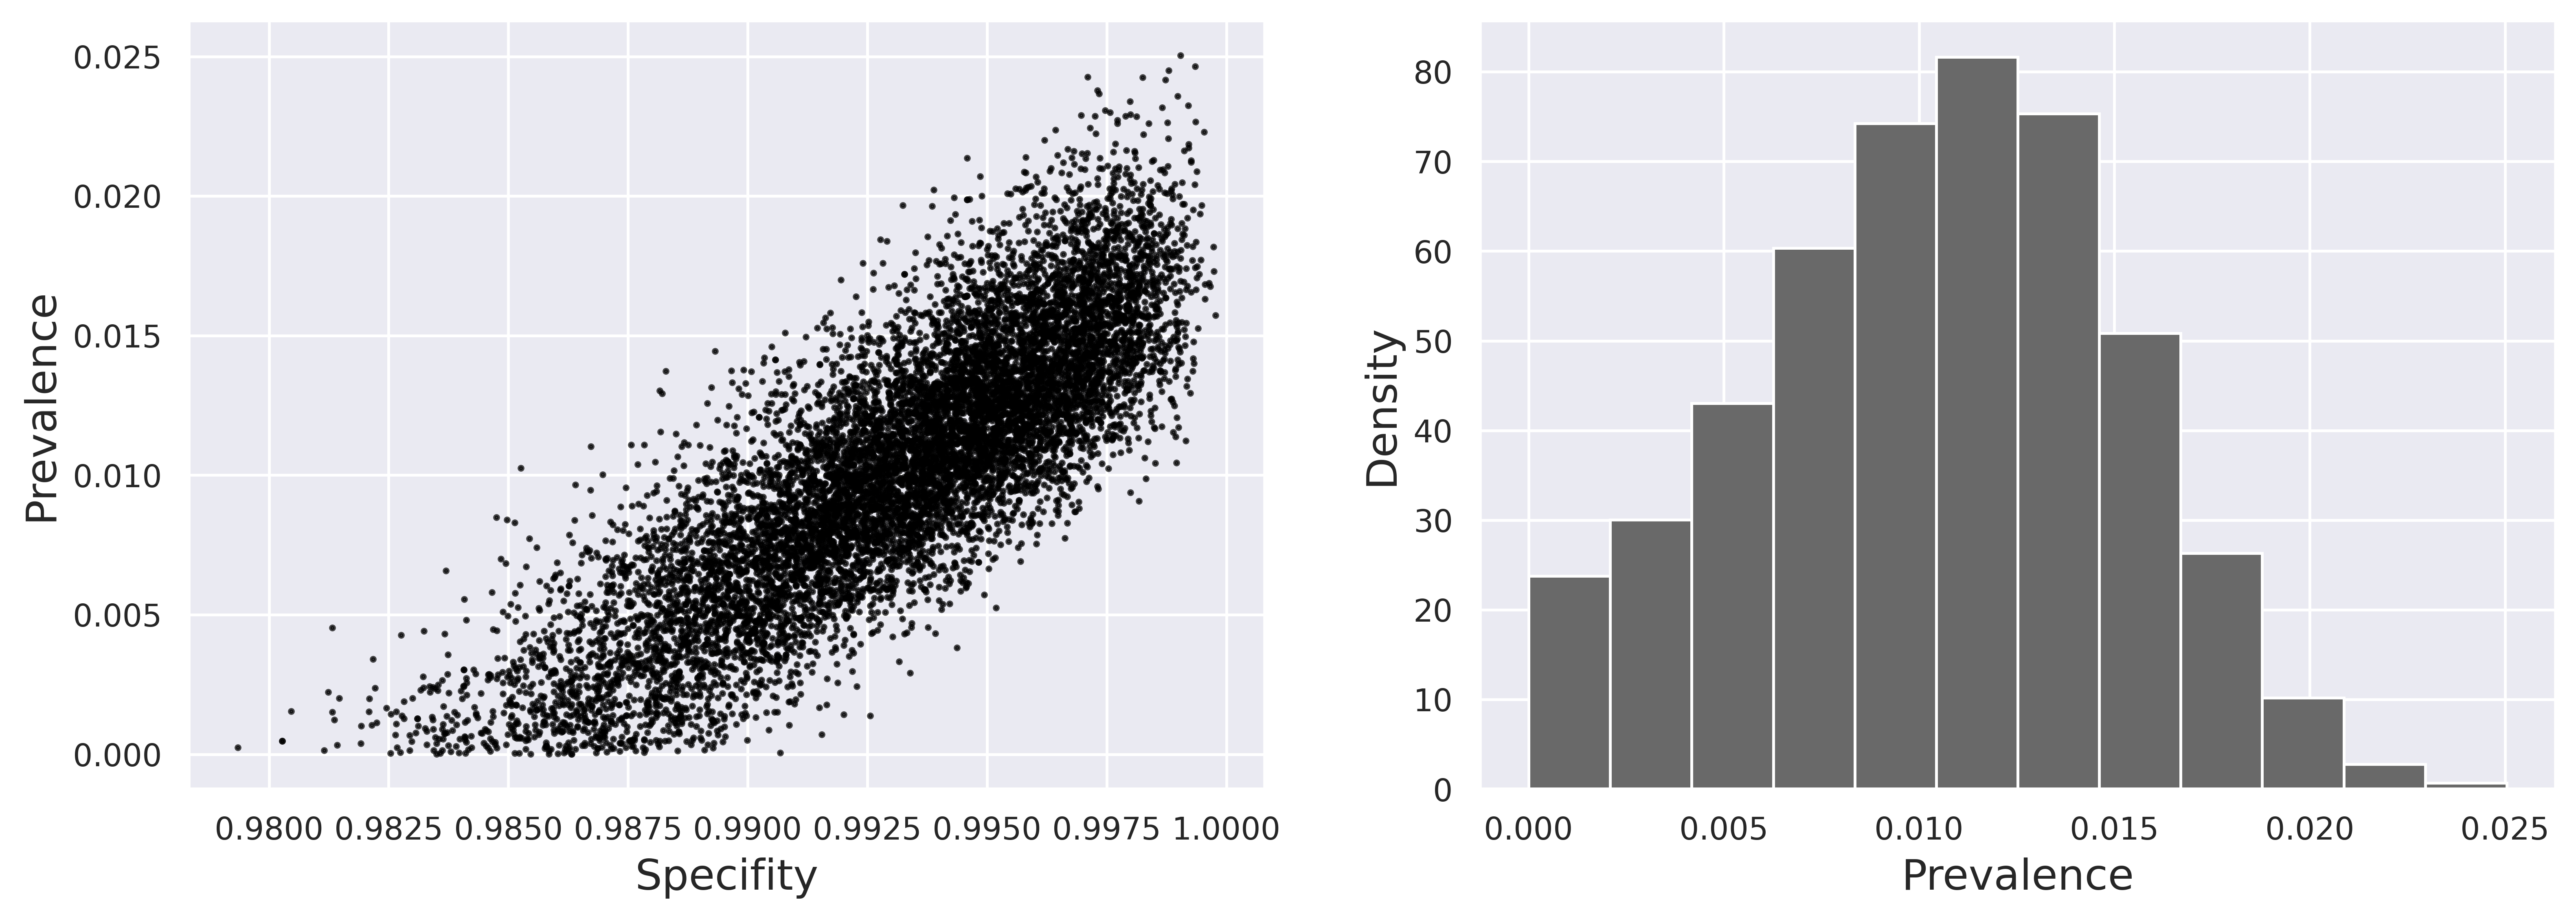
\includegraphics[width=\textwidth]{../../images/model1_gelman_figure_english.png}
  \caption{Scatter plot of posterior simulations of prevalence against
  specificity and histogram of posterior simulations of the prevalence.}
  \label{fig:results-posterior-model1}
\end{figure}

Other approach considers more than one study about specificity and
sensitivity. A {\em hierarchical partial pooling} model for these studies
can be done in the following way: 
\begin{gather*}
    \operatorname{logit}(\gamma_s^j) \sim \operatorname{Normal}(\mu_{\gamma_s}, \sigma_{\gamma_s}), \\
    \operatorname{logit}(\gamma_e^j) \sim \operatorname{Normal}(\mu_{\gamma_e}, \sigma_{\gamma_e}), 
\end{gather*}
for $1 \le j \le K$ studies, such that the first study is the considered one.
Partial pooling because the parameters can be sampled from the same
distribution. Hierarchical because the parameters of this distribution have
its one prior distributions. For instance, 
\begin{align*}
    \mu_{\gamma_s} &\sim N(0, 10), \\ 
    \mu_{\gamma_e} &\sim N(0, 10), \\
    \sigma_{\gamma_s} &\sim N^+(0,1), \text{ and } \\
    \sigma_{\gamma_e} &\sim N^+(0,1),
\end{align*}
where $N^+(a,b)$ is the truncated normal distribution in $[0,+\infty)$. All
the codes available at Github
repository\footnote{\url{https://github.com/lucasmoschen/rds-bayesian-analysis}}.

Finally, we studied a joint distribution for specificity and sensitivity, a
possible bivariate beta distribution built in \cite{olkin2015constructions}.
This distribution is derived from a Dirichlet distribution of order four. Let $U = (U[1],...,U[4]) \sim \operatorname{Dirichlet}(\boldsymbol{\alpha})$, where
$\boldsymbol{\alpha} \in \mathbb{R}^4_+$. Therefore, defining $X = U[1] +
U[2]$ and $Y = U[1] + U[3]$, we will have that $(X,Y)$ has a well-defined
probability distribution in
$[0,1] \times [0,1]$ such that $X$ and $Y$ have marginally beta distributions,
and they have correlation in all space. Depending on the definition of
$\boldsymbol{\alpha}$, the correlation between the variables range from -1 and
1. Figure \ref{fig:beta-bivariate} shows some examples of this construction. 

\begin{figure}[!ht]
    \centering
    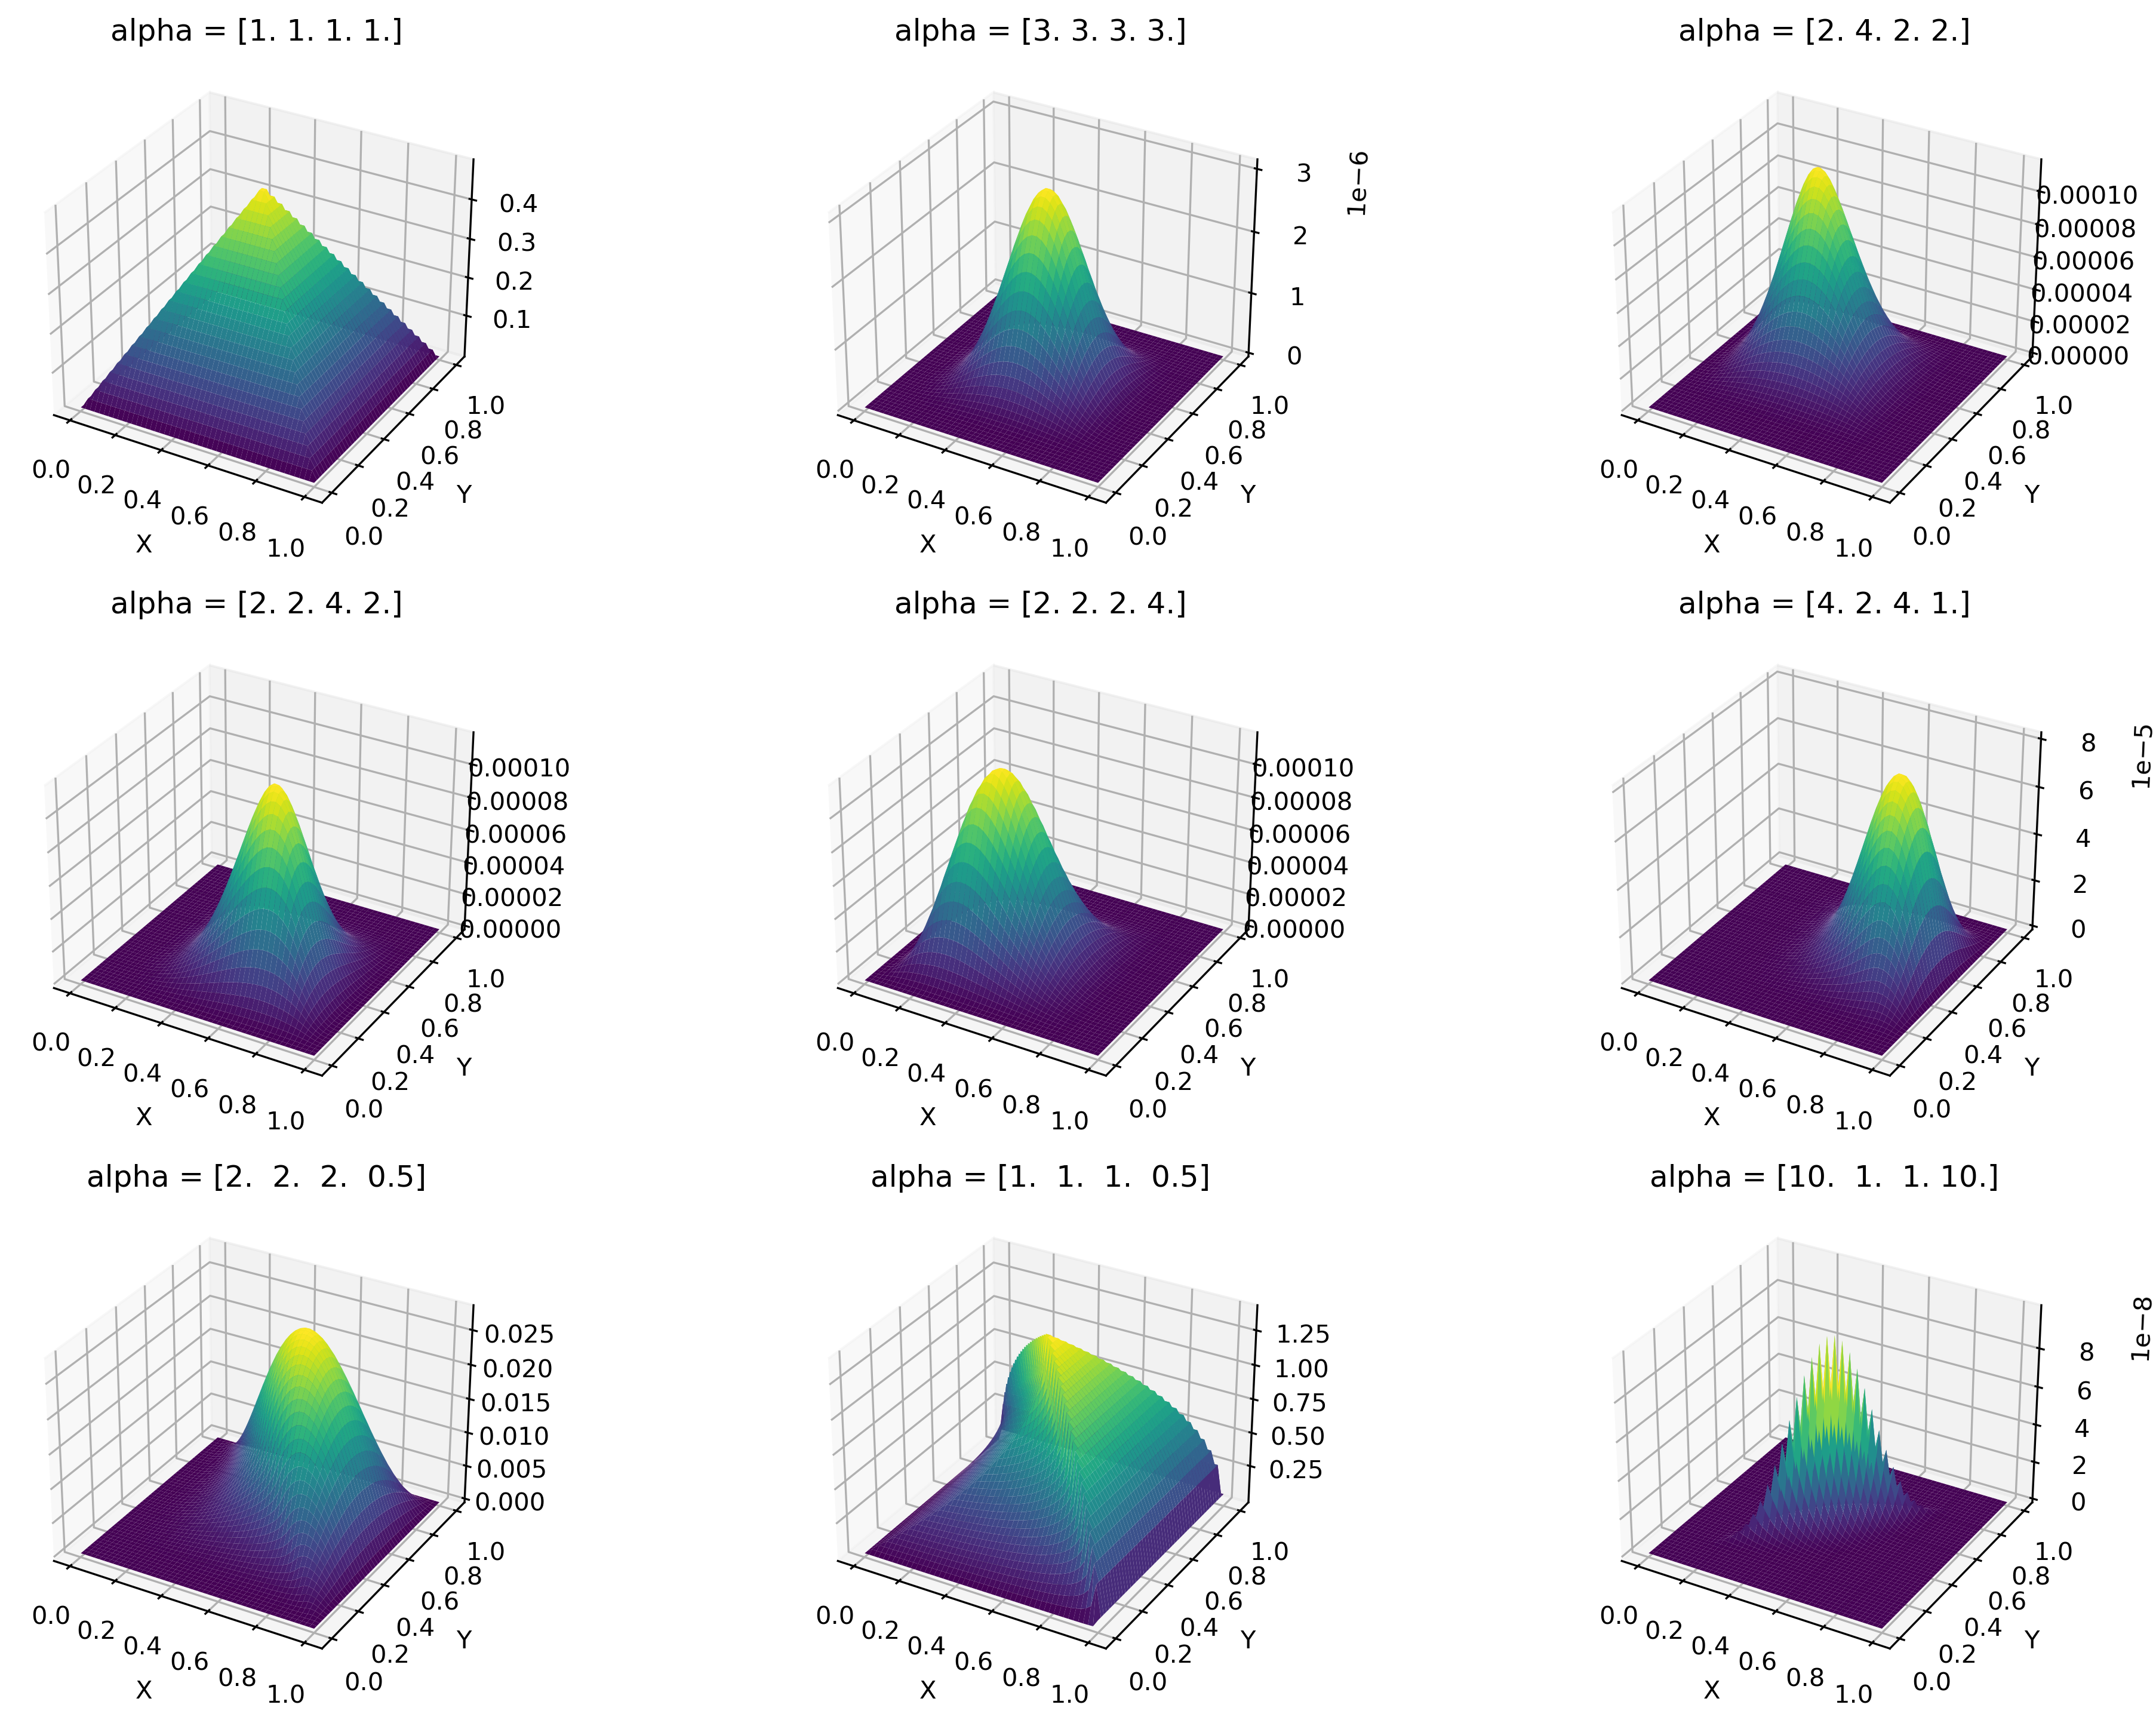
\includegraphics[width=\textwidth]{beta-distributions.png}
    \caption{Different choices of $\alpha$ and the joint distribution of the variables $X$ and $Y$.}
    \label{fig:beta-bivariate}
\end{figure}

\subsection{Imperfect tests and respondent-driven sampling}

For now, we consider the network dependence induced by the RDS with no
associated model. Therefore, we treat it as a random effect for
each individual. Conditionally autoregressive (CAR) models in the
Gaussian case are used. Let $[\tilde{Q}]_{ij} = \tilde{q}_{ij}$ be a fixed matrix which measures the distance between $i$
and $j$, and $\tilde{q}_{i+} = \sum_{j} \tilde{q}_{ij}$. In general, we use
$$
\tilde{q}_{ij} = \begin{cases}
  1, &\text{if } i \text{ recruited } j \text{ or the contrary} \\
  0, &\text{otherwise.} 
\end{cases}
$$
Next we define the scaled adjacency matrix $Q = D^{-1}\tilde{Q}$, such that $D$
is a diagonal matrix with $D_{ii} = \tilde{q}_{i+}$. Finally let $|\rho| < 1$ be a
parameter to controls the dependence between neighbors. Hence, we specify the
model as follows:

\begin{equation}
  \begin{aligned}
    T_i &\sim \bern(p_i) \\
    p_i &= \gamma_s\theta_i + (1-\gamma_e)(1 - \theta_i),  \\
    g(\theta_i) &= g(\theta) + \x_i^T\beta + \omega_i,  \\
    \omega_i|\{\omega_j\}_{j\neq i}, \tau &\sim \N\left(\rho\sum_j q_{ij}\omega_j, \tau^{-1}/\tilde{q}_{i+}\right) \\
    \beta &\sim \N(\mu, \Sigma), \\ 
    \theta &\sim \betadist(a^p, b^p) \\
    \gamma_s &\sim \betadist(a^s, b^s), \\
    \gamma_e &\sim \betadist(a^e, b^e), \\  
    \tau &\sim \operatorname{Gamma}(a^{\tau}, b^{\tau}).
  \end{aligned}  
\end{equation}
By Brook's Lemma \cite[]{brook1964distinction}, the joint distribution of
$\omega$ can be specified as 
$$
\omega \sim \N\left(0, \left[\tau (D - \rho \tilde{Q})\right]^{-1}\right).
$$

\subsubsection{Exponential Random Graph Model (ERGM)}

RDS has the constraint of being without replacement. For that reason, we do
not observe all links among the samples \cite[]{crawford2016}. Considering the
model developed by Crawford, we can model the
matrix $Q$ as {\em Exponential Random Graph Model} (ERGM). Define the
following 

\begin{enumerate}
  \item $\boldsymbol{s} = \tril(QC)^T \boldsymbol{1} + C^Tu$, such that $Q$ is the
  adjacency matrix of the recruited subjects, $C$ is the {\em Coupon Matrix},
  $u$ the vector of the number of edge ends belonging to each vertex
  (in the order of recruitment) that are not connected to any other sampled
  vertex, and $\tril(M)$ the lower triangle of $M$. 

  \item $T(Q) = -\lambda \boldsymbol{s}$, such that $\lambda$ is the rate of
  the recruitment time. 

  \item $V(Q) = \sum_{k \text{ is not seed}} \log(\lambda \boldsymbol{s}_k)$
  
  \item $w = (0, t_2 - t_1, ..., t_n - t_{n-1})$ is the vector of the waiting times between
  recruitments.  
\end{enumerate}

Therefore $\Pr(Q|w) \propto \exp[T(Q)^Tw + V(Q)]$. With that, the model
becomes 

\begin{equation}
  \begin{aligned}
    T_i &\sim \bern(p_i) \\
    p_i &= \gamma_s\theta_i + (1-\gamma_e)(1 - \theta_i),  \\
    g(\theta_i) &= g(\theta) + \x_i^T\beta + \omega_i,  \\
    \omega_i|\{\omega_j\}_{j\neq i}, \tau &\sim \N\left(\rho\sum_j q_{ij}\omega_j/q_{i+}, \tau^2/q_{i+}\right) \\
    Q|w &\propto \exp[T(Q)^Tw + V(Q)] \\
    \lambda &\sim \Gamma(a^{\lambda}, b^{\lambda}), \\ 
    \beta &\sim \N(\mu, \Sigma), \\ 
    \theta &\sim \betadist(a^p, b^p) \\
    \gamma_s &\sim \betadist(a^s, b^s), \\
    \gamma_e &\sim \betadist(a^e, b^e), \\  
    \tau &\sim \N^+(0,\sigma^2_{\tau}).
  \end{aligned}  
\end{equation}
The problem with this model is that we are assigning a posterior distribution
for $Q$.

% ----------------------------------------------------------
% Finaliza a parte no bookmark do PDF
% para que se inicie o bookmark na raiz
% e adiciona espaço de parte no Sumário
% ----------------------------------------------------------
\phantompart

\chapter{Conclusion}

\lipsum[1]

% ----------------------------------------------------------
% ELEMENTOS PÓS-TEXTUAIS
% ----------------------------------------------------------
\postextual
% ----------------------------------------------------------
---------------------------------------------------------
\bibliography{biblio}

% Consulte o manual da classe abntex2 para orientações sobre o glossário.
%
%\glossary

% ----------------------------------------------------------
% Apêndices
% ----------------------------------------------------------

% ---
% Inicia os apêndices
% ---
% \begin{apendicesenv}

% % Imprime uma página indicando o início dos apêndices
% \partapendices

% \end{apendicesenv}
% ---

% ----------------------------------------------------------
% Anexos
% ----------------------------------------------------------

% \begin{anexosenv}

% \partanexos

% \end{anexosenv}

%---------------------------------------------------------------------
% ÍNDICE REMISSIVO
%---------------------------------------------------------------------
\phantompart
\printindex

\end{document}